\newsection
\section{Рабочий проект}
\subsection{Модули, используемые при разработке сайта}

Интерфейс для врача или медсестры состоит из следующих компонентов

\begin{itemize}
	\item главное окно входа в систему;
	\item окно для регистрации нового пациента;
	\item форма регистрации нового пациента;
	\item форма регистрации нового врача;
	\item регистрационная форма для специальности ``Hematology'';
	\item регистрационная форма для специальности ``Immunology'';
	\item регистрационная форма для специальности ``Urine Analysis'';
	\item регистрационная форма по специальности ``Fecal Analysis'';
	\item регистрационная форма по специальности ``Serology'';
	\item регистрационная форма по специальности ``Microbiology''.
\end{itemize}

Модули классифицируются на формы, соединения и ввод базы данных.
В таблице \ref{table:modd} описаны модули и функции для формы врача.

\begin{xltabular}{\textwidth}{|p{2.5cm}|p{2.5cm}|p{4.85cm}|p{4.85cm}|}
\caption{Спецификация модуля ``Doctors''.\label{table:modd}}\\
\hline \centrow Название класса & \centrow Модуль, к которому относится класс & \centrow Описание класса & \centrow Методы \\
\hline \centrow 1 & \centrow 2 & \centrow 3 & \centrow 4\\
\endfirsthead
\caption*{Продолжение таблицы \ref{table:modd}}\\
\hline \centrow 1 & \centrow 2 & \centrow 3 & \centrow 4\\
\finishhead
\hline
cont\_form & doctors.php & cont\_form - для создания нового медицинского учреждения, и с необходимыми разрешениями для входа в систему сайта, вместе с методом post для чтения того, что написано в форме. & <class="cont\_form"> <class="head"> <h1>NewDoctror</h1> <method\=``post'' action=``/admin/ Save\_d.php''> \\ \hline
\end{xltabular}

В таблице \ref{table:modp} описывает модули и функции формы пациента.

\begin{xltabular}{\textwidth}{|p{2.5cm}|p{2.5cm}|p{4.85cm}|p{4.85cm}|}
\caption{Спецификация модуля ``Patient''.\label{table:modp}}\\
\hline \centrow Название класса & \centrow Модуль, к которому относится класс & \centrow Описание класса & \centrow Методы \\
\hline \centrow 1 & \centrow 2 & \centrow 3 & \centrow 4\\
\endfirsthead
\caption*{Продолжение таблицы \ref{table:modp}}\\
\hline \centrow 1 & \centrow 2 & \centrow 3 & \centrow 4\\
\finishhead
\hline
cont\_form & Patient.php & cont\_form -  помогает создать новую запись со всеми личными данными пациента, зарегистрированного в медицинской лаборатории. & <class="cont\_form"> <class="head"> <h1>NewPatient</h1> <method\=``post'' action=``/admin/ Save\_p.php''> \\ \hline
\end{xltabular}

В таблице \ref{table:moda} описаны модули и функции формы для всех специальностей медицинской лаборатории.

\begin{xltabular}{\textwidth}{|p{2.5cm}|p{3cm}|p{4.85cm}|p{4.85cm}|}
\caption{Спецификация модуля ``Analysis''.\label{table:moda}}\\
\hline \centrow Название класса & \centrow Модуль, к которому относится класс & \centrow Описание класса & \centrow Методы \\
\hline \centrow 1 & \centrow 2 & \centrow 3 & \centrow 4\\
\endfirsthead
\caption*{Продолжение таблицы \ref{table:moda}}\\
\hline \centrow 1 & \centrow 2 & \centrow 3 & \centrow 4\\
\finishhead
\hline
form\_grup & formulario.php & form\_grup -  Это класс, который поможет в создании формы для специальностей, которые есть в медицинской лаборатории. & <method=``post''  ``action=''<?php echo \$action ;?>"> \\ \hline
\end{xltabular}

Все модули работают с одним и тем же соединением с базой данных. В следующей таблице \ref{table:consa} указаны формы и типы подключения к базе данных.

\begin{xltabular}{\textwidth}{|p{2.5cm}|p{3cm}|p{4.85cm}|p{4.85cm}|}
\caption{Спецификация модуля ``Conexion'' и ``Save''.\label{table:consa}}\\
\hline \centrow Название класса & \centrow Модуль, к которому относится класс & \centrow Описание класса & \centrow Методы \\
\hline \centrow 1 & \centrow 2 & \centrow 3 & \centrow 4\\
\endfirsthead
\caption*{Продолжение таблицы \ref{table:consa}}\\
\hline \centrow 1 & \centrow 2 & \centrow 3 & \centrow 4\\
\finishhead
\hline
conexion & Conexion.php & conexion - В этом классе есть все поля валидации для правильного входа на сервер, в базу данных и таблицы. &  \$pdo=newPDO ("mysql:host={\$config ['host']};dbname= {\$config['dbname']}
\$config['user'], 
\$config['password']) \\ \hline
\end{xltabular}

Каждый модуль сохранения имеет соединение с базой данных. В следующей таблице \ref{table:save} указаны формы и типы каждого сохранения для информации, зарегистрированной в каждой форме.

\begin{xltabular}{\textwidth}{|p{2.5cm}|p{3cm}|p{4.85cm}|p{4.85cm}|}
	\caption{Спецификация модуля ``Conexion'' и ``Save''.\label{table:save}}\\
	\hline \centrow Название класса & \centrow Модуль, к которому относится класс & \centrow Описание класса & \centrow Методы \\
	\hline \centrow 1 & \centrow 2 & \centrow 3 & \centrow 4\\
	\endfirsthead
	\caption*{Продолжение таблицы \ref{table:save}}\\
	\hline \centrow 1 & \centrow 2 & \centrow 3 & \centrow 4\\
	\finishhead
	\hline
	Save analysis & Save\_a.php & Save analysis - это класс, который помогает хранить данные, введенные для каждой специальности, в каждой выделенной таблице. &  \$statement = \$conn->prepare('INSERT INTO specialty (columns) VALUES (values)');\\ \hline
	Save doctors & Save\_d.php & Save doctors - это класс, который поможет вам сохранить введенные данные для новых врачей. &  \$statement = \$conn->prepare('INSERT INTO doctors (columns) VALUES (values)');\\ \hline
	Save patient & Save\_p.php & Save patient - это класс, который поможет вам сохранить данные, введенные для новых пациентов, поступивших в медицинскую лабораторию. &  \$statement = \$conn->prepare('INSERT INTO patient (columns) VALUES (values)');\\ \hline
\end{xltabular}

Для представления данных в табличной форме вызывается модуль ``Show'', который считывает данные, введенные для пациентов в медицинской лаборатории. В следующей таблице \ref{table:info} показан модуль запроса к базе данных.

\begin{xltabular}{\textwidth}{|p{2.5cm}|p{3cm}|p{4.85cm}|p{4.85cm}|}
	\caption{Спецификация модуля ``Information''.\label{table:info}}\\
	\hline \centrow Название класса & \centrow Модуль, к которому относится класс & \centrow Описание класса & \centrow Методы \\
	\hline \centrow 1 & \centrow 2 & \centrow 3 & \centrow 4\\
	\endfirsthead
	\caption*{Продолжение таблицы \ref{table:info}}\\
	\hline \centrow 1 & \centrow 2 & \centrow 3 & \centrow 4\\
	\finishhead
	\hline
	Show & Show.php & Show - это класс, который помогает сделать запрос к таблице принятых пациентов и отобразить на веб-странице медицинской лаборатории. &   \$sql ='SELECT * FROM dbo.Patients';
	\$result = mysqli\_query(\$link, \$sql);
	 if (\$result == false) {
		print( mysqli\_error(\$link));}\\ \hline
\end{xltabular}

\subsection{Описание объектов интерфейса программы}

Начиная с дизайна интерфейса, описанного в пункте 2.3 технической спецификации, php и css использовались в качестве языков стилей вместе с программой Visual Studio Code 2022 для разработки интерфейса для пользователя, который будет иметь доступ ко всей информации медицинской лаборатории, и который сможет вести учет пациентов. формы веб-страницы.

На рисунке \ref{img:pagp} вы можете увидеть графическое представление интерфейса, где показаны различные поля и соответствующие кнопки. Цветные прямоугольники, представленные на рисунке, используются для идентификации различных объектов, составляющих интерфейс.

Исходный код программы, реализующей этот программный интерфейс, представлен в \hyperref[ПРИЛОЖЕНИЕ]{приложение Б} как часть документации.

\subsection{Модульное тестирование разработанного web-сайта}

Тестирование модулей проводилось с использованием языка стилей CSS для лучшего распознавания мест для форм, размещения и связывания каждой из них с ее кодировкой.

Модуль проверяет валидность пользователей и паролей врачей \ref{image:codus}.

\begin{figure}
\begin{lstlisting}[language=html]
session_start();
if (!empty($_POST['username']) && !empty($_POST['password'])) {
	require '../admin/Conexion.php';
	$conn = conexion($config);
	$username = $_POST['username'];
	$password = $_POST['password'];
	$records = $conn->prepare('SELECT id, username, password FROM doctors WHERE username = :username');
		$records->bindParam(':username', $username);
	$records->execute();
	$results = $records->fetch(PDO::FETCH_ASSOC);
	$message = "";
	if (count($results) > 0 && $_POST['password'] == $results['password']) {
		$_SESSION['user_id'] = $results['id'];
		header("Location: ../");
	} else {
		$message = "Sorry, those credentials do not match";}}?>
\end{lstlisting}

\caption{Модульный пользователей и паролей врачей}
\label{image:codus}
\end{figure}

\subsection{Системное тестирование разработанного web-сайта}

Случай использования: домашняя страница;
Предусловие: браузер закрыт;
Тестовый случай: вход на сайт медицинской лаборатории;
Ожидаемый результат: браузер открыт, страница загружена.

На рисунке \ref{image:log} показана главная страница сайта для ввода имени пользователя и пароля врача.

\begin{figure}
\center{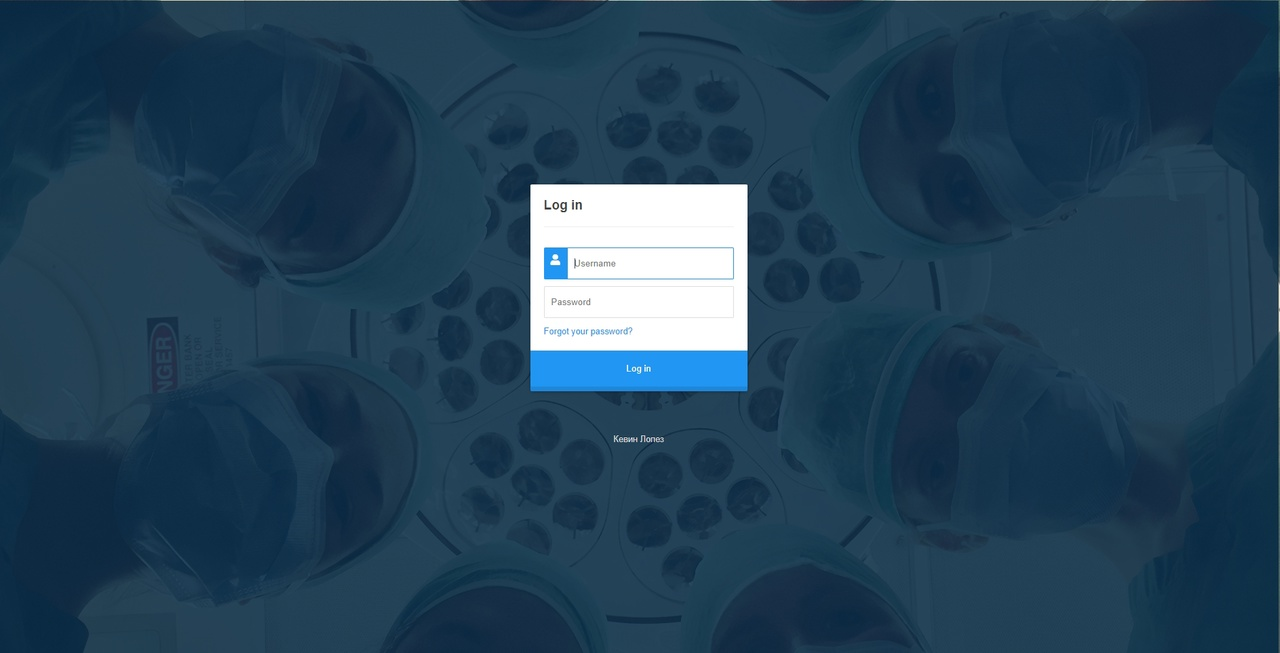
\includegraphics[width=1\linewidth]{Login}}
\caption{Главная страница сайта для ввода имени пользователя и пароля}
\label{image:log}
\end{figure}

Случай использования: пользователь или пароль не вошли в систему;
Предусловие: открыта домашняя страница;
Тестовый случай: логин или пароль врача;
Ожидаемый результат: система показывает ошибку при вводе имени пользователя или пароля.

Если имя пользователя или пароль неверны, веб-страница будет перенаправлена на окно ошибки, как показано на рисунке \ref{image:error}.

\begin{figure}
	\center{
\includegraphics[width=0.3\linewidth]{error}}
	\caption{Окно ошибки}
	\label{image:error}
\end{figure}

Сайт содержит навигационное меню с левой стороны, которое облегчает врачу поиск специальностей или регистрацию нового врача или пациента.
На рисунке \ref{image:menu} показана страница с навигационным меню.

\begin{figure}
	\center{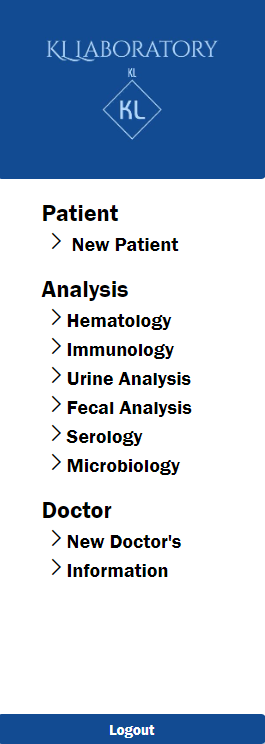
\includegraphics[width=0.2\linewidth]{menu}}
	\caption{Меню навигации}
	\label{image:menu}
\end{figure}

Случай использования: прием нового пациента;
Предусловие: эффективная валидация имени пользователя и пароля;
Тестовый случай: заполнение формы для регистрации нового пациента;
Ожидаемый результат: форма заполнена и эффективно зарегистрирована в базе данных.

На рисунке \ref{image:pac} показана страница с формой регистрации пациентов для приема в медицинскую лабораторию.

\begin{figure}
	\center{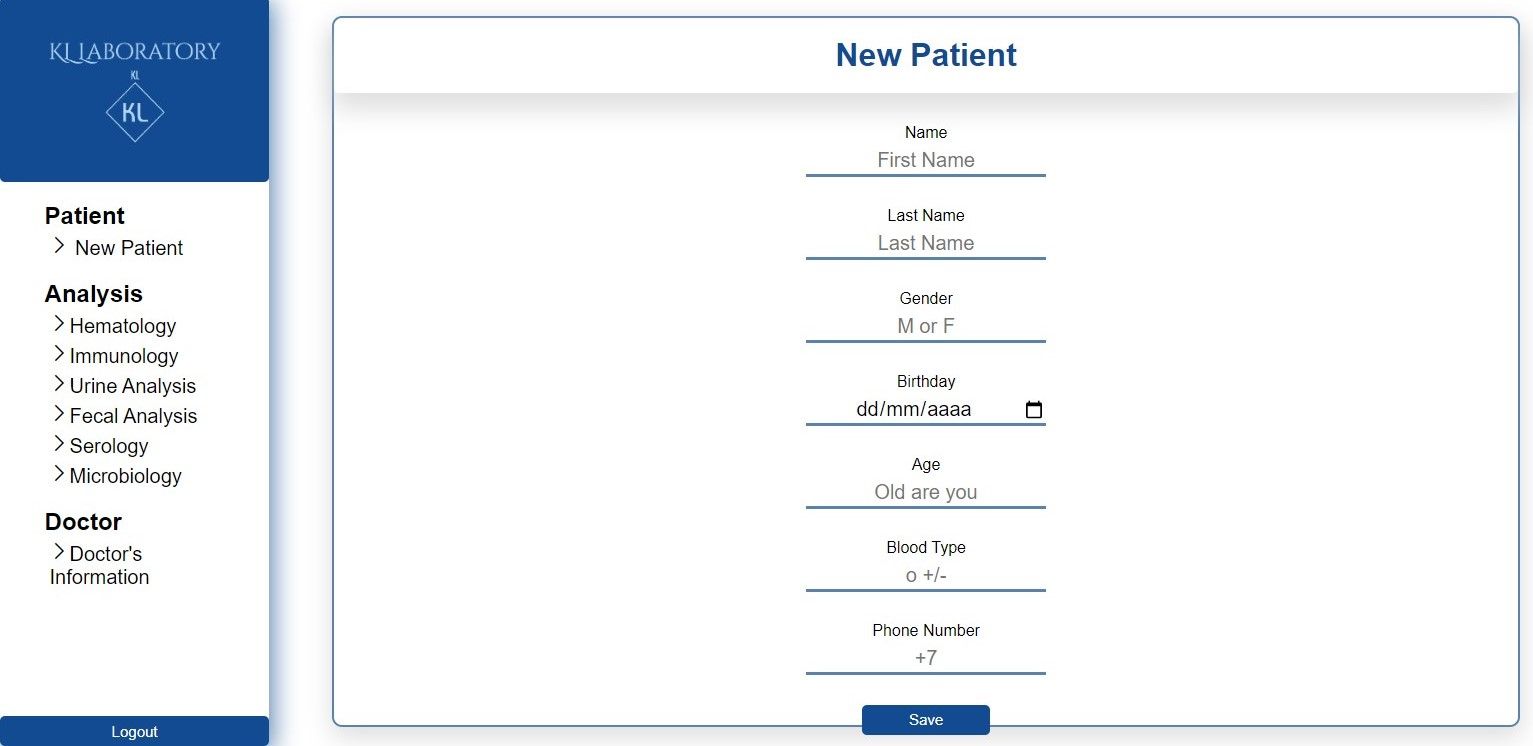
\includegraphics[width=1\linewidth]{pagi1}}
	\caption{Форма для нового пациента}
	\label{image:pac}
\end{figure}

Случай использования: вход в систему нового врача;
Предусловие: пользователь выбирает в навигационном меню регистрацию нового врача;
Тестовый случай: заполнение формы для регистрации нового врача;
Ожидаемый результат: форма заполнена и эффективно зарегистрирована в базе данных.

На рисунке \ref{image:doc} показана страница с регистрационной формой для новых врачей, поступающих в медицинскую лабораторию.

\begin{figure}
	\center{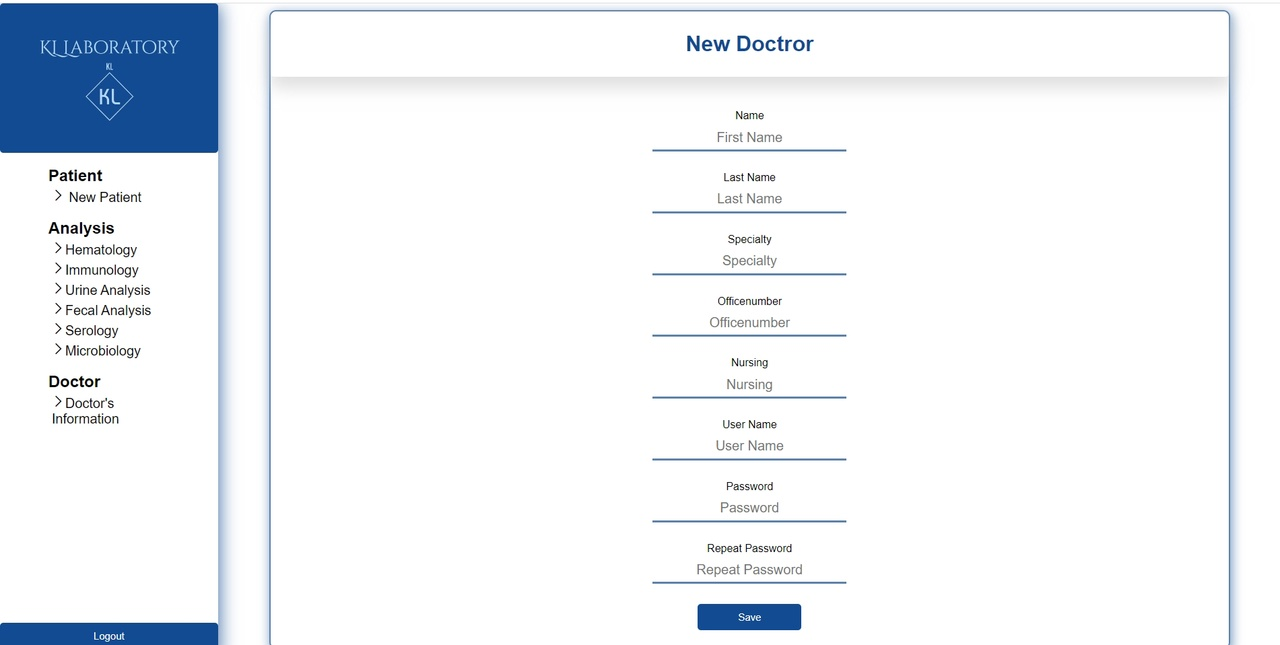
\includegraphics[width=1\linewidth]{pag3}}
	\caption{Форма нового врача}
	\label{image:doc}
\end{figure}

Случай использования: регистрация процессов и обследований пациентов;
Предусловие: пользователь выбирает в навигационном меню специальность для регистрации пациента;
Тестовый случай: заполнение формы с процедурами, результатами и лечением пациента;
Ожидаемый результат: заполненная форма и эффективная регистрация в базе данных в таблице каждой специальности.

На рисунке \ref{image:ana} показана страница с регистрационной формой для одной из специальностей медицинской лаборатории.

\begin{figure}
	\center{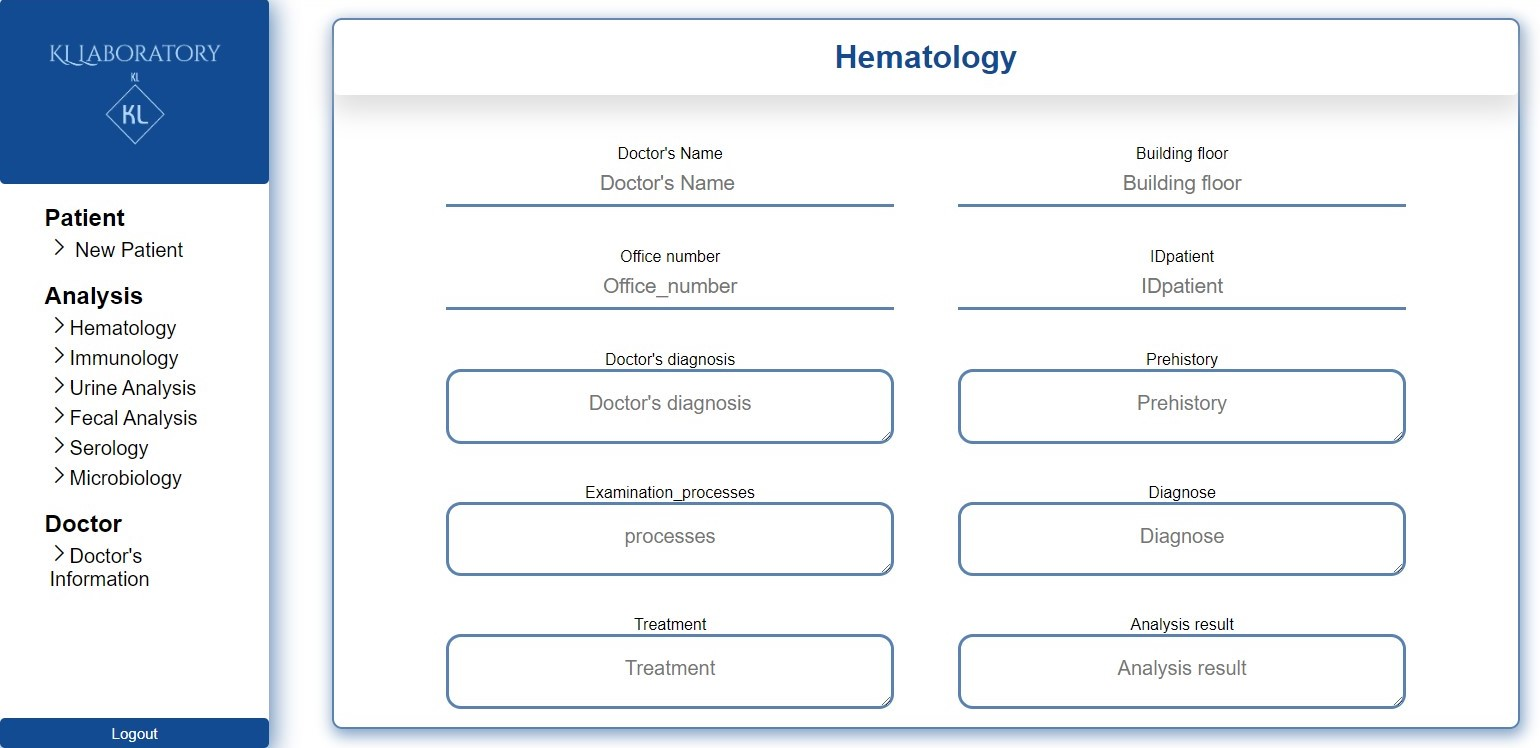
\includegraphics[width=1\linewidth]{pag2}}
	\caption{Форма специализации}
	\label{image:ana}
\end{figure}

Случай использования: верификация пациентов в системе;
Предусловие: пользователь выбирает опцию информации в навигационном меню;
Тестовый случай: визуализация таблицы с записями пациентов, внесенными в базу данных;
Ожидаемый результат: отображение таблицы со всей информацией о пациентах, внесенной в медицинскую лабораторию.

На рисунке \ref{image:infor} показана страница базы данных с информацией о пациенте.

\begin{figure}
	\center{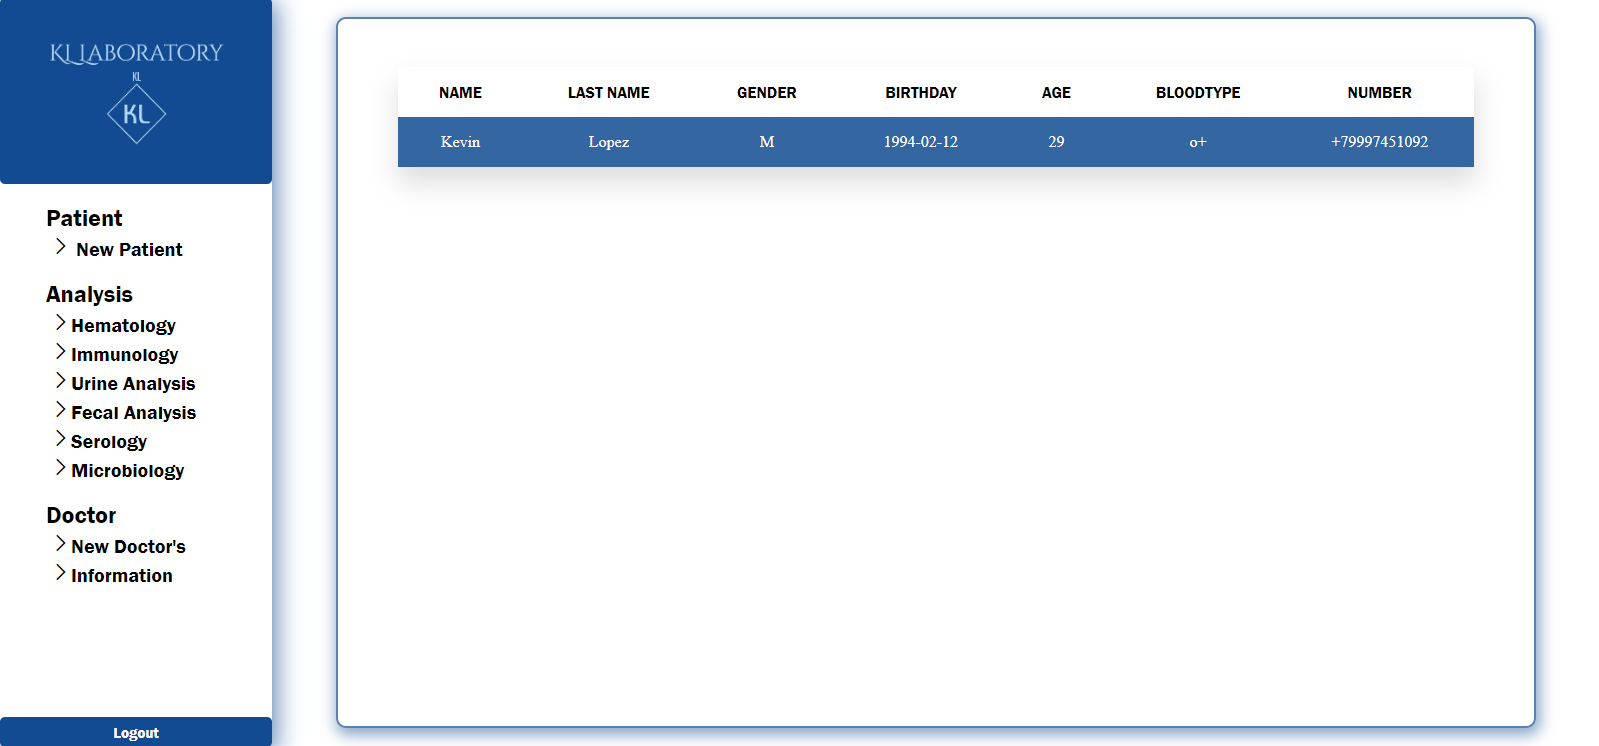
\includegraphics[width=1\linewidth]{inform}}
	\caption{Пациенты, зарегистрированные в базе данных}
	\label{image:infor}
\end{figure}

\subsection{Тестирование интерфейсов в среде веб-страницы}

Пример пользовательского тестирования, включающий запуск и навигацию по веб-странице, будет использован для объяснения процесса разработки наборов тестов для интерфейсов.

В таблице \ref{table:test} показаны различные тестовые наборы для проверки функциональности пользовательского интерфейса во время его запуска и отладки.

\begin{xltabular}{\textwidth}{|X|X|X|X|}
	\caption{Тестовые наборы для отладки интерфейса веб-сайта медицинской лаборатории.\label{table:test}}\\
	\hline \centrow Проверяемая ситуация & \centrow Действия пользователя & \centrow Входные данные & \centrow Реакция системы \\
	\hline \centrow 1 & \centrow 2 & \centrow 3 & \centrow 4\\
	\endfirsthead
	\caption*{Продолжение таблицы \ref{table:test}}\\
	\hline \centrow 1 & \centrow 2 & \centrow 3 & \centrow 4\\
	\finishhead
	\hline
	Пользователь не ввел имя пользователя или пароль в начальное поле. & Пользователь не вводил цифры, символы или буквы в поля логина и пароля врача. & Поле ввода имени пользователя и пароля пусто. & Система отображает временное сообщение
	``введите имя пользователя и пароль''.\\ \hline
	Перейти на главную страницу. & Пользователь правильно введите имя пользователя и пароль врача. & Пользователь правильно вводит данные врача, а затем нажимает кнопку для входа в систему. & Система я открываю главную страницу, которая является формой для регистрации нового пациента.\\ \hline
	Регистрация нового пациента. & Пользователь заполняет поля формы. & Врач или медсестра вводит личную информацию пациента, который собирается поступить в медицинскую лабораторию.Затем нажмите кнопку сохранить. & Система проверяет информацию, введенную в поля формы для записи в таблицу базы данных.\\ \hline
	Заполнение специальной формы. & Пользователь выбирает специальность в лаборатории. & Врач или медсестра выбирают специальность, необходимую пациенту, и записывают проводимые с ним процедуры и обследования.Затем нажмите кнопку сохранить. & Система проверяет и записывает информацию, введенную в поля формы, и сохраняет в табеле каждой специальности в базе данных.\\ \hline
	Регистрация нового врача. & Пользователь регистрирует нового врача в медицинской лаборатории. & Врач или медсестра запишут информацию о новом враче, который будет работать в медицинской лаборатории. А затем нажмите кнопку сохранения. & Система проверяет информацию и заносит в таблицу врачей в базе данных.\\ \hline
	Отображать информацию. & Пользователь хочет видеть информацию о пациентах. & В информационном поле отображается табала со всеми личными данными пациентов, зарегистрированных в медицинской лаборатории. & Система развертывает таблицу, выполняя запрос из базы данных.\\ \hline 
	Выход из системы & Пользователь желает покинуть сеанс врача. & Пользователь нажимает кнопку выхода в нижней части меню навигации. & Система завершает сеанс и возвращается на главный экран, чтобы снова ввести имя пользователя и пароль.\\ \hline	
\end{xltabular}